\section{Апробация}
\label{sec:testing}

\subsection{Тестовое окружение}

В качестве основной конкретной реализации \ukanren для тестирования
использовался OCanren\footnote{https://github.com/JetBrains-Research/OCanren}\cite{ocanren},
реализованный на OCaml\cite{ocanren}.
Для некоторых тестов для использовался faster-miniKanren\footnote{https://github.com/miniKanren/faster-miniKanren},
версия miniKanren, реализованная на Scheme.

Тесты запускались на обычном ноутбуке: Intel Core i5-6200U CPU, 2.30GHz, DDR4, 12GiB.

Для тестирования суперкомпилятора и его модификаций использовался следующий алгоритм.
\begin{enumerate}
\item Подготавливается программа, реализованная на внутреннем представлении \ukanren.
\item Программа и запрос, на который будет происходит специализация, подаются на вход суперкомпилятору.
\item По дереву процессов, порождённому суперкомпилятором, строится остаточная программа.
\item Остаточная программа транслируется в OCanren/faster-miniKanren и
      запускается в заранее подготовленном окружении с тестовыми запросами.
\end{enumerate}


Реализованный суперкомпилятор сравнивался с реализацией \forcpd для $\mu$Kanren\footnote{\url{https://github.com/kajigor/uKanren_transformations}},
а также c реализацией \forcpd для Prolog --- системой ECCE\footnote{\url{https://github.com/leuschel/ecce}}.
Другие специализаторы не рассматриваются, так как согласно работе~\cite{controlPoly}, специализация с
помощью \cpd в ECCE показывает лучшие результаты.

Для последнего требовалось оттранслировать программу на \ukanren в Prolog, специализировать
её на запрос, далее оттранслировать результирующую программу в OCanren.
Это допустимо сделать в силу того, что между \ukanren и подмножеством Prolog есть
взаимооднозначное соответствие. 
Все необходимые средства для этого также предоставлялись указанной библиотекой специализации.


\subsubsection{Набор тестов}

Набор мелких тестов на базовую валидацию сгенерированных программ.

\begin{itemize}
 \item Программа \rel{doubleAppend}(xs, ys, zs, rs), которая
       производит конкатенацию трёх списков. Она классически используется
       для проверки эффекта дефорестации в специализированной программе.
 \item Программа \rel{maxLen}(xs, max, len), которая находит в списке
       максимальный элемент и длину списка. Она классически используется
       для проверки эффекта таплинга в специализированной программе. 
 \item Программа сортировки \rel{sort}(list, result). Выбрана в силу показательности
       результатов.
%     Запросы:
%     \begin{itemize}
%     \item оптимизация сортировки: \rel{sort}(xs, ys);
%     \item генерация отсортированных последовательностей: \rel{sort}(xs, xs).
%     \end{itemize}
% \item Отношение, проверяющее принадлежность пути графу \rel{isPath}(path, graph, result).
%       Специализация \rel{isPath}(path, graph, true). Запросы:
%     \begin{itemize}
%     \item генерация $n$ произвольных путей в случайном графе;
%     \item поиск пути заданного размера в случайном графе: \\ $\text{isPath}^o_s$(p, g)$\land$\rel{length}(p, N).
%     \end{itemize}
 \item Интерпретатор формул логики высказываний \rel{logint}(formula, subst, result).
       Интерпретатор специализируется на то, чтобы всегда генерировать выполнимые формулы
       \rel{logint}(formula, subst, true).
%      Запросы:
%     \begin{itemize}
%     \item поиск $n$ решений заданной формулы;
%     \item генерация $n$ формул с подстановке размера $n$.
%     \end{itemize}
% \item Интерпретатор лямбда-исчисления \rel{lam}(expr, result). Запросы:
% 	\begin{itemize}
% 	\item генерация $n$ выражений в нормальной форме \rel{lam}(expr, expr);
% 	\item генерация $n$ выражений, редуцирующихся к заданному выражению \rel{lam}(expr, E).
% 	\end{itemize}
% \item Проверка типов в просто типизировнном лямбда-исчислении \rel{infer(type, expr)}.
%     \begin{itemize}
% 	\item Поиск $n$ обителей заданного типа.
% 	\item Генерация выражений, соответствующих заданной спецификации типа и выржения. Специализируется выражение:\\
% 	      \rel{infer}(type, expr) $\land$ type $\equiv$ TYPE\_SPEC $\land$ expr $\equiv$ EXPR\_SPEC.
%     \end{itemize}
% \item Интерпретатор простого подмножества Scheme.
%    \begin{itemize}
%    \item \todo{Интересный тест!}
%    \end{itemize}
\end{itemize}

% \subsection{Апробация базового суперкомпилятора \ukanren}
% % Для начала разберём, как базовый суперкомпилятор ведёт себя на
% базовом наборе программ, результат которых несложно проанализировать.

% \begin{itemize}
% \item Классическая программа \lstinline{doubleAppend}~\cite{cpd}, которая используется для
%       проверки наличия эффекта дефорестации (\todo{В приложении}).
% %\item Другая классическая программа \lstinline{maxLength}~\cite{cpd}, которая
% %      используется для проверки наличия эффекта таплинга.
% \end{itemize}

Разберём на примере результат работы базового суперкомпилятора.

Классическая программа для тестирования эффектов специализации ---
\lstinline{doubleAppend}, представленная на рисунке~\ref{fig:dappCode},
в которой происходит конкатенация списков трёх списков.

\begin{figure}[h!]
\begin{lstlisting}
doubleAppend a b c d =
  fresh (t)
   (append a b t $\land$ append t c d)
append y4 y5 y6 =
  (y4 $\equiv$ [] $\land$ y6 $\equiv$ y5) $\lor$
  fresh (ty t h)
   (y4 $\equiv$ h :: t $\land$
    y6 $\equiv$ h :: ty $\land$
    append t y5 ty)
\end{lstlisting}
\caption{Программа для тестирования \lstinline{doubleAppend}}
\label{fig:dappCode}
\end{figure}

Во многих бенчмарках~\cite{cpdPract, controlPoly} это программа используется
для проверки эффекта дефорестации.

Рассмотрим дерево процессов на рисунке~\ref{fig:dappTree}
(для компактности \lstinline{append} сокращён до \lstinline{app}),
которое порождается применением базового
суперкомпилятора к программе \lstinline{doubleAppend}, причём в
качестве аргументов --- простые свободные переменные, из-за чего
просто оптимизируется сама структура программы.

\begin{figure}[h!]
\center
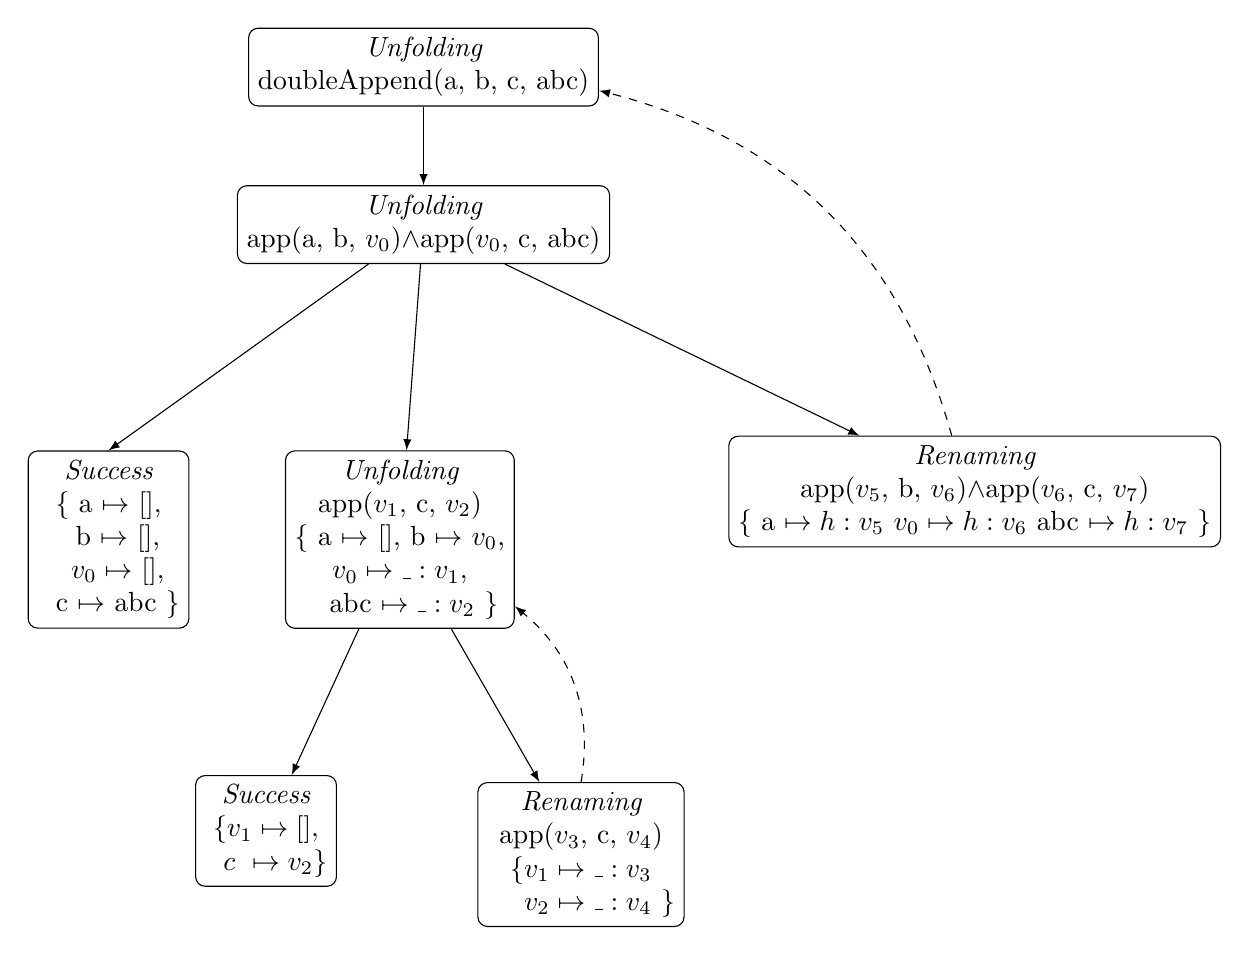
\begin{tikzpicture}[->,node distance=3cm, sibling distance=6.2cm, level distance=2cm]
  \tikzstyle{conf}=[rectangle,draw, rounded corners=.8ex,align=center]
  \node[conf] (root)   at (0, 0)     {{\it Unfolding} \\ \lstinline{doubleAppend(a, b, c, abc)}};
  \node[conf] (appapp) at (0, -2)    {{\it Unfolding} \\ \lstinline{app(a, b, $\text{v}_0$)$\land$app($\text{v}_0$, c, abc)}};
  \node[conf] (app1)   at (-0.3, -6) {{\it Unfolding} \\ \lstinline{app($\text{v}_1$, c, $\text{v}_2$)} \\ $\{$ a $\mapsto$ [], b $\mapsto$ $\text{v}_0$, \\ $\text{v}_0 \mapsto \_ : \text{v}_1$, \\ $\ \ $ abc $\mapsto \_ : \text{v}_2$ $\}$};
  \node[conf] (app2)   at (7, -5.39) {{\it Renaming} \\ \lstinline{app($\text{v}_5$, b, $\text{v}_6$)$\land$app($\text{v}_6$, c, $\text{v}_7$)} \\ $\{$ a $\mapsto \text{h} : \text{v}_5$  $\text{v}_0 \mapsto \text{h} : \text{v}_6 $  abc $\mapsto \text{h} : \text{v}_7$  $\}$};
  \node[conf] (appS)   at (-4,-6)    {{\it Success} \\ $\{$ a $\mapsto$ [], \\ \ \ b $\mapsto$ [],\\ \ \ $\text{v}_0 \mapsto$ [], \\ \ \ c $\mapsto$ abc $\}$};
  \node[conf] (app11)  at (2,  -10)  {{\it Renaming} \\ \lstinline{app($\text{v}_3$, c, $\text{v}_4$)} \\ $\{\text{v}_1 \mapsto \_ : \text{v}_3 $ \\ $\ \ \ \ \text{v}_2 \mapsto \_ : \text{v}_4 $  $\}$};
  \node[conf] (app1S)  at (-2, -9.7) {{\it Success} \\ $\{ \text{v}_1 \mapsto [],$ \\ $\ \ c \ \mapsto \text{v}_2 \}$};
  \draw[-latex] (root) -- (appapp);
  \draw[-latex] (appapp) -- (appS.north);
  \draw[-latex] (appapp) -- (app1);
  \draw[-latex] (appapp) -- (app2);
  \draw[-latex] (app1) -- (app1S);
  \draw[-latex] (app1) -- (app11);
  \draw[-latex,dashed] (app2) edge [bend right] (root);
  \draw[-latex,dashed] (app11) edge [bend right] (app1);
\end{tikzpicture}
\caption{Дерево процессов для программы \lstinline{doubleAppend}}
\label{fig:dappTree}
\end{figure}

В приведённом дереве первым этапом происходит замена определения \lstinline{doubleAppend}
на его тело. Так как в определении нет дизъюнкий, получаем всего одну конфигурацию,
в которой операцией \lstinline{fresh} добавляется новая семантическая переменная $\texttt{v}_0$.
Далее происходит обработка конфигурации с более чем одним конъюнктом. Так как используется
полная стратегия развёртывания, каждая из конъюнкий раскрывается по определению и
рассматривается их дизъюнктивная нормальная форма, в которой всего четыре дизъюнкта,
один из которых не унифицируется, поэтому всего появляется только три конфигурации.
Эти конфигурации рассматривают несколько возможных значений переменных:
\begin{enumerate}
\item когда \lstinline{a} и \lstinline{b} пустые списки, то результатом конкатенации
является \lstinline{c};
\item если же \lstinline{b} не пуст, тогда результат --- это конкатенация списков \lstinline{b} и \lstinline{c}.
      Отношение конкатенации двух списков также специализируется под задачу.
      В результате этой специализации порождается исходное отношение, поскольку
      никакой новой информации не было выявлено и исходная программа уже была оптимальна;
\item в третьем же случае выводится, что результат конкатенации трёх списков
      \lstinline{a}, \lstinline{b} и \lstinline{c} --- это конкатенация
      списков $\texttt{v}_5$, \lstinline{b} и \lstinline{c}, где $\texttt{v}_5$
      является хвостом списка, а в голову которой добавили голову \lstinline{a}.
\end{enumerate}

По данному дереву порождается остаточная программа, изображённая на рисунке~\ref{fig:dappCodeOpt}.
\begin{figure}[h!]
\begin{lstlisting}
doubleAppendo a b c d =
  fresh (x4) (app3 a b x4 c d)
app3 a b t c d =
   fresh (x7 x6 x5 x10 x9 x8)
     (a $\equiv$ [] $\land$ b $\equiv$ t $\land$
       (t $\equiv$ [] $\land$ c $\equiv$ d $\lor$
       (t $\equiv$ x8 :: x9) $\land$
        d $\equiv$ x8 :: x10 $\land$
        app2 x9 c x10
     ) $\lor$
     (a $\equiv$ x5 :: x6 $\land$
      t $\equiv$ x5 :: x7 $\land$
      d $\equiv$ x5 :: x10 $\land$
      app3 x6 b x7 c x10) ) 
app2 a b c =
  fresh (x13 x12 x11)
   (a $\equiv$ [] $\land$ b $\equiv$ c $\lor$
   (a $\equiv$ x11 :: x12 $\land$
    c $\equiv$ x11 :: x13 $\land$
    app x12 b x13))
\end{lstlisting}
\caption{Суперкомпилированная программа \lstinline{doubleAppend}}
\label{fig:dappCodeOpt}
\end{figure}

В итоге, наблюдается, как двупроходный алгоритм становится однопроходным.


\subsection{Сравнение вариаций суперкомпилятора \ukanren}

В таблице~\ref{fig:dappTest} представлены результаты сравнения модификаций
с базовым суперкомпилятором при разных стратегиях развёртывания.
При полных стратегиях для doubleAppendo возникает эффект дефорестации.
В остальных стратегиях этого не происходит, из-за чего исполнения по
крайней мере в два раза хуже. Из-за того, что программа довольно небольшая,
модификации алгоритма суперкомпиляции хотя не оказывают влияния не результат.

\begin{table}[h!]
\center
\begin{tabular}{|l|c|c|c|c|c|}
\hline
   &     1   &    2   &      3 &    u   &   u2 \\ \hline
FU & 0.0040 & 0.0041 &0.0040 & 0.0042 &0.0040  \\ \hline
FnU& 0.0040 & 0.0037 &0.0039 & 0.0039 &0.0040  \\ \hline
SU & 0.0099 & 0.0093 &0.0094 & 0.0096 &0.0127  \\ \hline
NU & 0.0097 & 0.0096 &0.0100 & 0.0097 &0.0097  \\ \hline
RU & 0.0096 & 0.0094 &0.0096 & 0.0099 &0.0092  \\ \hline
MnU& 0.0097 & 0.0103 &0.0097 & 0.0095 &0.0096  \\ \hline
MxU& 0.0110 & 0.0096 &0.0095 & 0.0094 &0.0094  \\ \hline
FsU& 0.0095 & 0.0096 &0.0099 & 0.0092 &0.0098  \\ \hline
\end{tabular}
\caption{Результат для doubleAppendo c конкатенацией трёх списков длины 120, секунды}
\label{fig:dappTest}
\end{table}

В таблице~\ref{fig:maxlenTest} указаны результаты тестирования для
программы maxLength. 

\begin{table}[h!]
\center
\begin{tabular}{|l|c|c|c|c|c|}
\hline
   &     1    &    2   &       3 &    u   &   u2 \\ \hline
FU & 0.1152 & 0.0457 &  0.1090 & 0.0448 & 0.0457 \\ \hline
FnU& 0.1064 & 0.1070 &  0.1035 & 0.0437 & 0.0485 \\ \hline
SU & 0.0497 & 0.0485 &  0.0479 & 0.0495 & 0.0472 \\ \hline
NU & 0.0483 & 0.0475 &  0.0484 & 0.0466 & 0.0487 \\ \hline
RU & 0.1564 & 0.0999 &  0.1491 & 0.0993 & 0.0973 \\ \hline
MnU& 0.0489 & 0.0480 &  0.0479 & 0.0474 & 0.0485 \\ \hline
MxU& 0.0481 & 0.0472 &  0.0478 & 0.0478 & 0.0484 \\ \hline
FsU& 0.1485 & 0.1006 &  0.1479 & 0.1587 & 0.1608 \\ \hline
\end{tabular}
\caption{Запуск для maxLength, секунды}
\label{fig:maxlenTest}
\end{table}

\begin{table}[h!]
\center
\begin{tabular}{|l|c|c|c|c|c|}
\hline
   &     1    &    2   &       3 &    u   &   u2   \\ \hline
FU & 0.2634   & 0.2587 & 0.2596  & 0.2577 & 0.2515 \\ \hline
FnU& 0.2591   & 0.2552 & 0.2505  & 0.2581 & 0.2524 \\ \hline
SU & 0.2525   & 0.2541 & 0.2501  & 0.2509 & 0.2638 \\ \hline
NU & 0.2601   & 0.2560 & 0.2617  & 0.2550 & 0.2628 \\ \hline
RU & 0.2633   & 0.2606 & 0.2591  & 0.2662 & 0.2681 \\ \hline
MnU& 0.2655   & 0.2603 & 0.2606  & 0.2721 & 0.2613 \\ \hline
MxU& 0.2726   & 0.2682 & 0.2570  & 0.2515 & 0.2571 \\ \hline
FsU& 0.2632   & 0.2525 & 0.2613  & 0.2559 & 0.2603 \\ \hline
\end{tabular}
\caption{Запуск для sort}
\end{table}

\begin{table}[h!]
\center
\begin{tabular}{|l|c|c|c|c|c|}
\hline
   &     1    &    2   &       3 &    u   &   u2    \\ \hline
FU &    -     & 0.1318 &    -     & 0.1049 &    -   \\ \hline
FnU& 0.0716   & 0.2097 & 0.0765   & 0.1115 & 0.1258 \\ \hline
SU & 0.1811   & 0.1491 & 0.1681   & 0.0902 & 0.0913 \\ \hline
NU & 0.0921   & 0.1356 & 0.0778   & 0.0883 & 0.1144 \\ \hline
RU & 0.0740   & 0.0954 & 0.0816   & 0.0637 & 0.1263 \\ \hline
MnU& 0.0639   & 0.1097 & 0.0802   & 0.0921 & 0.1170 \\ \hline
MxU& 0.1929   & 0.1438 & 0.1644   & 0.0775 & 0.1108 \\ \hline
FsU& 0.1636   & 0.1757 & 0.1807   & 0.0701 & 0.1894 \\ \hline
\end{tabular}
\caption{Запуск для loginto subst0}
\end{table}
